 \chapter{Technical Analysis} \label{TechAnalysis}
 
The work cell regarding this project, consists of a number of machines and other articles used in the production of a rotor for one of the pumps at Grundfos. This chapter provides a description of these articles and their function in the work cell\cite{robotsave}. All the measurements noted in this analysis is based on the scale, which has been provided in the case description see \cite{Case}, due to the lack of information of the machine dimensions. \\ 
 


 \section{Work-cell}
 The rotor arrives in the work-cell on a conveyor see \ref{fig:Layoutworkcell}, the rotor always has the same orientation and stops in same position, the conveyor has a sensor that activates a hardware pin when a new rotor is in place.\\
 The manipulator's control box then receives a signal from the sensor, which tells the manipulator the rotor is at the given position, then the can process begin.\\
%\begin{figure}[H]
%    \centering
%   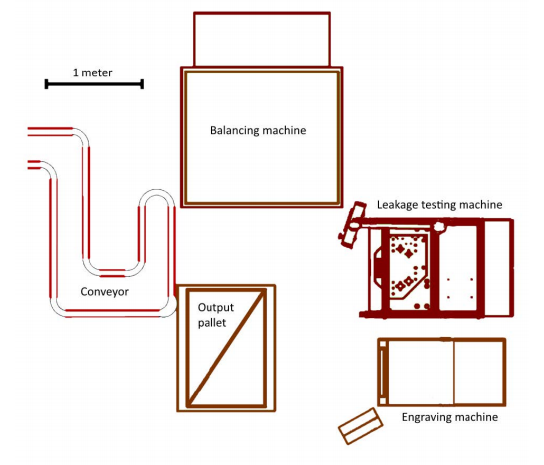
\includegraphics[width=\textwidth]{TechnicalAnlysis/layout.PNG}
%    \caption{Preliminary layout of work-cell\cite{Case}}
%    \label{fig:Layoutworkcell} 
%\end{figure}

%\begin{figure}[H]
%    \centering
%    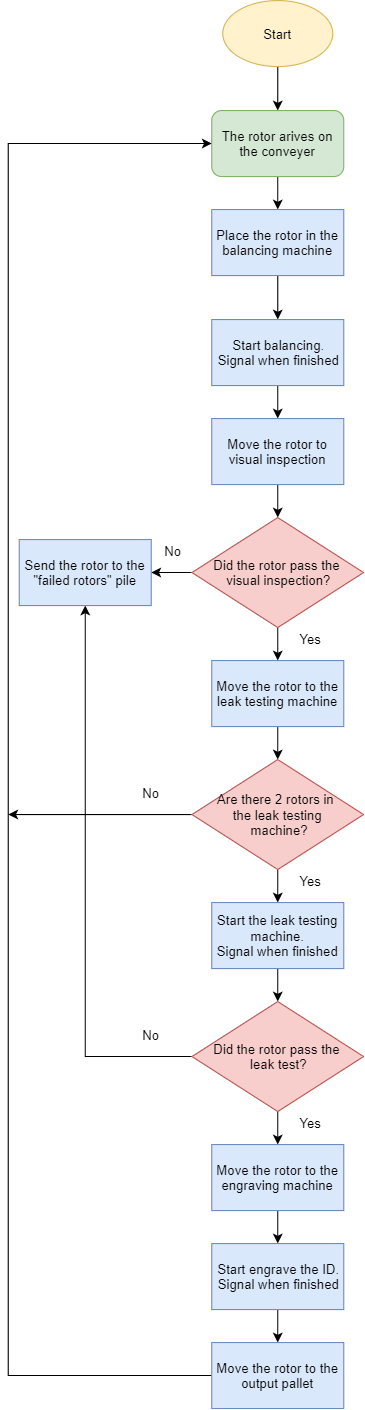
\includegraphics[width=0.4\textwidth]{InitialProblemstatement/Case/UMLcasenyeste.PNG}
%    \caption{A preliminary flow chart based on the case}
%    \label{fig:caseflow}
%\end{figure}

\begin{tikzpicture}[node distance=2cm]


\node (start) [startstop] {The rotor arrives on conveyer};

\node (pro1) [process, below of=start, yshift=-1cm] {The rotor is moved to balancing machine, and balancing commences};
\node (pro2) [process, below of=pro1, yshift=-2cm] {The rotor is moved to visual inspection, and visual inspection commences};

\node (dec1) [decision, below of=pro2, yshift=-2.3cm] {Did the rotor pass visual inspection?};
\node (out1) [io, right of=dec1, xshift=3.5cm] {Move the rotor to failed pile};
\node (stop) [startstop, below of=dec1, yshift=-2cm] {The rotor is moved to the queue table};

\draw [arrow] (start) -- (pro1);
\draw [arrow] (pro1) -- (pro2);
\draw [arrow] (pro2) -- (dec1);

\draw [arrow] (dec1) -- node[anchor=south] {no} (out1);
\draw [arrow] (dec1) -- node[anchor=east] {yes} (stop);


\end{tikzpicture}




\begin{tikzpicture}[node distance=2cm]


\node (start) [startstop] {The rotor arrives on the queue table};
\node (pro1) [process, below of=start, yshift=-0.8cm] {The rotor is moved to the leakage testing machine};

\node (dec1) [decision, below of=pro1, yshift=-2cm] {Are there 2 rotors in the LTM?};
\node (out1) [io, right of=dec1, xshift=4cm] {Perform the previous tasks until another rotor is available};
\node (pro2) [process, below of=dec1, yshift=-1.4cm] {Leakage testing commences};

\node (dec2) [decision, below of=pro2, yshift=-1.4cm] {Did the rotor pass leakage testing?};
\node (out2) [io, right of=dec2, xshift=3.5cm] {Move the rotor to failed pile};
\node (pro3) [process, below of=dec2, yshift=-2.5cm] {The rotor is moved to the engraving machine, and engraving commences};

\node (stop) [startstop, below of=pro3, yshift=-1.2cm] {The rotor is moved to output pallet};


\draw [arrow] (start) -- (pro1);
\draw [arrow] (pro1) -- (dec1);

\draw [arrow] (dec1) -- node[anchor=south] {no} (out1);
\draw [arrow] (dec1) -- node[anchor=east] {yes} (pro2);

\draw [arrow] (pro2) -- (dec2);

\draw [arrow] (dec2) -- node[anchor=south] {no} (out2);
\draw [arrow] (dec2) -- node[anchor=east] {yes} (pro3);

\draw [arrow] (pro3) -- (stop);

\end{tikzpicture} 

 


%\subsection{The ideal work-cell}
%The ideal work-cell would only require having a single robot manipulator to move the rotor between all the stations.\\
%The setup for the ideal work-cell has to consider several parameters.\\ 
%First parameter is to find a layout that has the least amount of open floor space.\\
%Second, is it possible to arrange the setup differently, so the robot manipulator will be able to reach more locations, without having to move.\\
%Third, consider whether it is more effective to use more than one robot manipulator, rather than having it mounted on a moving platform.
 
 \subsection{Balancing machine}
 The rotor has to be placed in the balancing machine see \ref{fig:balancing}, this is done via a drawer, see \ref{fig:Rotor} that opens and closes automatically, so a signal that tells if the drawer is opened or closed is needed to verify the status of the drawer. A signal from the manipulator to the balancing machine is needed so the manipulator can signal the machine to close its drawer and begin balancing.\\
 
\begin{figure}[H]
\centering
    \begin{subfigure}{.49\textwidth}
        \centering
        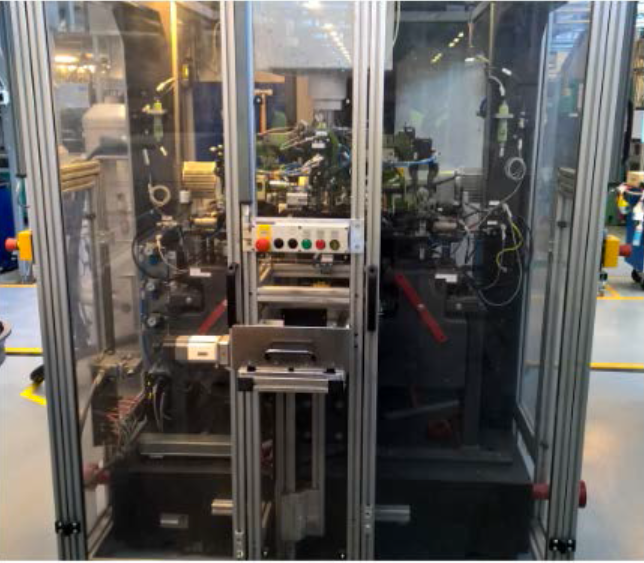
\includegraphics[width=\textwidth]{InitialProblemstatement/Case/balancing.PNG} 
        \caption{Balancing machine overview}
        \label{fig:balancing}
    \end{subfigure}
    \begin{subfigure}{.49\textwidth}
        \centering
        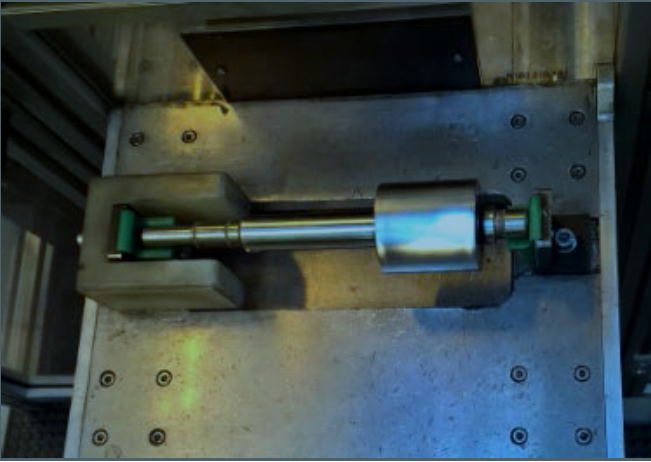
\includegraphics[width=\textwidth]{InitialProblemstatement/Case/Rotor.PNG}
        \caption{Balancing machine drawer with L40 rotor}
        \label{fig:Rotor} 
    \end{subfigure}
\caption{Balancing machine\cite{Case}}
\label{fig:BalancingMachine}
\end{figure}
\\
The balancing machine is 1.65m in width and 2.0m in length.\\
The balancing machine is only capable of testing 1 rotor at a time.\\
The machine consists of 2 rigid pedestals, with bearings and suspension on the top, supporting a mounting platform where the rotor will be placed hanging on the pedestals.\\
The test will function by the machine turning the rotor, while a vibration sensor detects differences of unbalance in the rotor. From that information it can tell where to add or remove weights, to balance the rotor, after which a visual inspection is required. \\
Safety measures might have to be taken, if an employee has to enter the work-space to inspect the rotor. \\

 \subsection{Leak testing machine}
 
 The leak testing machine, see \ref{fig:Leak testing machine} is 1.2m wide (with control pad), and 1.8m of length.\\ 
 It is used to test the rotors for a leakage, and it can hold up to 2 rotors per test.\\
 The rotor is placed standing upright with the longest part of the ensemble facing in to the hole of the cylinder. Then the leak machine will pressurize the rotor to a preset.\\
 The transducer inside the leak machine will be put into a zero state, and the different pressures will be applied. After stabilization the rotor will then be compared to the transducer towards the different pressure volumes, if the volumes differ too much an alarm limit will be triggered, and the visual signal lights will light red and await for an operator to re-activate it again. \\
 When the rotor passes, a green light will indicate the pass and the hatches around the rotor will be released and the pressure will be stabilized to the normal atmosphere  \cite{LEAK},\cite{LEAK2}. \\
 The UR5 needs to point the rotors in a 45 degree manner when inserting it into the cylinder, so that the rotor can be placed with a sliding trajectory. \\
 
 \begin{figure}[H]
    \centering
    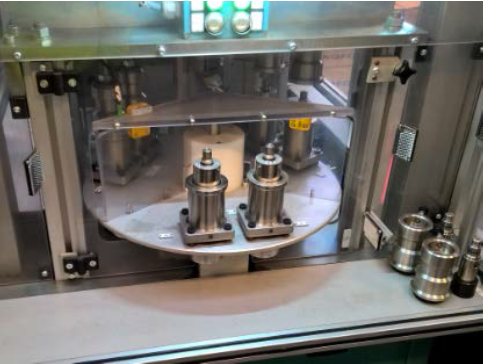
\includegraphics[width=9cm]{InitialProblemstatement/Case/Leaktest.PNG}
    \caption{The leak testing machine\cite{Case}}
    \label{fig:Leak testing machine}
\end{figure}
 
 \subsection{Laser engraver}
 Before the rotor can be placed in the fixture of the engraving machine see \ref{fig:Laserengravermachine}, there is a need to check if there is already a rotor in the fixture or the rotor needs to be temporarily store at the buffer table. If the fixture is empty, the manipulator can place the rotor in the fixture, the rotor needs to place up side down in engraver. When the rotor is placed, the manipulators control box has to send a signal to the engraving machine that tells that it can begin the process. When the engraving is done a signal has to be send to the control box, that tells that the engraving machine is finished marking the rotor and can be stored on the pallet.\\
 The engraving machine has a dimension of 0,7m width and 1,3m in length. \\
 It is used to engrave the part number ID of the rotor, there is space for one rotor per cycle.\\
 The engraver is made with a laser engraver from ROFIN, it uses a set of mirrors to control the laser beam\cite{laser}. The rotor is placed in a fixture inside the engraving machine, with a screen that protects people from the harmful laser beam, has to be closed, this can be done from a foot pedal. When the engraving is done the screen opens and the rotor can be stored at the pallet. \\   
  
  \begin{figure}[h]
    \centering
    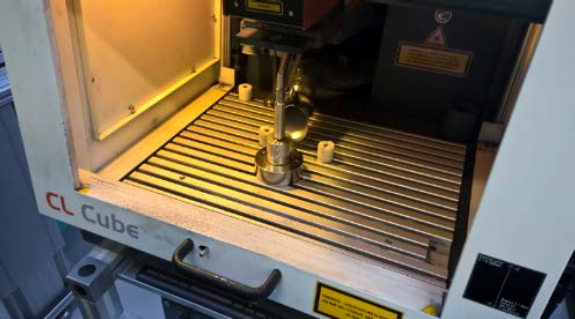
\includegraphics[width=9cm]{InitialProblemstatement/Case/engrave.PNG}
    \caption{Laser engraver machine\cite{Case}}
    \label{fig:Laserengravermachine}
  \end{figure}
  
 \subsection{Queue table}
 The queue table is a box with holes that serves as a temporary storage for the rotors. Up to 100 rotors can be placed here at any given point during the process to rest, and then be moved to the appropriate machine when they are ready. The queue table has a length and width of 51.5 cm. and a height of 80 cm\cite{Case}.\\  
 
 \subsection{Output pallet}
 When the rotors are complete, they can be moved to the output pallet, which can hold up to 320 rotors at a time. When the pallet is full, an employee will replace it with an empty pallet \cite{Case}.\\ 
 
\subsection{Degrees of Freedom}\label{DOFSec}

To pick and place the rotors, a manipulator must have a certain number of DOF (degrees of freedom). The minimum required DOF to lift and move an object is 3, since the cartesian space of the x,y and z, makes the movement of the object from point 1 to point 2 without changing the objects orientation and only moving it in a 2d space. Take for example a 1 DOF robot, this would only be able to move the object in a curved line.\\
The UR5 has 6 DOF, and can therefore move an object to any point within a 3-dimensional space. It can also apply pitch, roll and yaw to an object, thereby allowing it to rotate the object in any direction\cite{DOF}. \\ 
In the work-cell which this project concerns, at least 6 DOF are required, since it is required to move the rotors around in the work-cell, as well as up and down, in order to pick them up, move them to a new location and place them down. It is also needed to rotate the rotors to the appropriate orientation before placing them. 

\paragraph{Fixtures and holders:} There has to be made some assumption on the fixtures and holders, to plan for a robot that has a high enough accuracy to place the rotor in the position and orientation. The team made the assumption that fixtures and holder has tolerance of 1 mm when inserting a rotor. 

 
 \section{Possible work-cell sensors}\label{ref:PlacementS}
 
 When the robot needs to operate inside the work-cell, it needs to have some sensors in place which will tell it when to pick and place the rotor.\\
 By taking the machines, as seen above into consideration, communication between the machines and the manipulator is a must.\\
 Here are some possible solutions:\\

 
  \subsection{LIDAR} 
  LIDAR sensors can be used to determine the object position spot inside the work-cell, some LIDARs project a 3D point cloud and others work in a 2D-plane\cite{LIDAR}.\\
  The 3D LIDAR can be used to create a 3D representation of the work cell.A 2D LIDAR can be used as distances measurement device. It can measure the distance in the field of view depending on the product\cite{LIDAR}.\\

 % \subsection{Force sensor} \label{pressure}
  %Pressure sensors which are included in the cobot, can be used as a weight distributor. Where the cobots payload of the rotor will be released when placed, and then the pressure sensor on the machines, could determine whether it was placed correctly.\\
 
  \subsection{Photocell sensors} 
  Photo-cell sensors can be used to signal that the rotor is in the right place on the conveyor. The photocell works by sending either infrared light or visible light, from a transmitter to a receiver, or some photocells work by setting up a mirror that reflects the light from the transmitter back to itself. If an object breaks the light beam, a hardware pin goes high or low depending on the type of sensor\cite{SICKfo}.\\

 \subsection{Inductive sensor}
 Inductive sensors can only detect metal, but it has an advantage over the capacities sensors, since it has a further detection range. The inductive sensors from SICK, which have a detection range from 20mm to 60mm \cite{SICKin} where a capacities sensor max range is from 16mm to 25mm \cite{SICKka} that could be found, so the range and distance of the inductive sensor can be better. Some inductive sensors can also give an analog signal so that these sensors can detect how far the metallic object is from the sensor\cite{SICKin}.\\ 

 \subsection{Capacities sensor} 
 Capacities sensors works much in the same ways as the inductive sensor, but they can detect metal and non metallic objects.\cite{SICKka}.\\

 \subsection{Depth sensing camera} \label{depthcam}
 Depth sensing Cameras can be used as means to give the manipulator a vision over the work-cell, by determining a position of the object in references to the end-effector\cite{cam}. This can be done through the use of the inverse kinematic, here it is needed to calculate frame reference from the base to the camera, so it can compute the coordinates from the camera and find the angles of joints to reach the object\cite{JohnC}.\\


 %3. All of the above could be managed with the interface of ROS, where a service program could be included to send messages through the topics of both cobot and machine. Hereby the two collaborating systems could interact between each other and send commands that could be interpreted by the cobot.\\ 
 
 %3.Industrial robots might use extra safety precautions, to decrease the probability of incidents happening. This could be extra sensors detecting when humans enter, or leave their designated work-space. For caged robots, the door to the cage must usually be closed in order for the robot to run, but you might also want other more reactive ways of ensuring the safety of the personal, particularly when using collaborative robots. One of the most used sensors on these kind of robots would be a collision detection sensor. This allows the robot to register when colliding with a soft surface, and the ability to then either stop, or reduce speed.\\ 

%Many other types of safety sensors might be needed when humans are working side by side with robots. This could include cameras, lasers or pressure sensors. Anything that can help letting the robots know, that humans are present.\\ 

%When working in a production, that require the robots to pick up parts, and place them elsewhere, it might be a very good idea to have a part detection sensor. This sensor tells the robot whether it picked something up or not, and potentially if it is picked up in the right way. If something goes wrong, the robot might either send an error message to an operator, or try to repeat the task, depending on the configuration\cite{sensors}.\\ 


%Although the technical minimum requirement to solve the tasks is only 4 DOF, having more gives the robotic manipulator more flexibility, thereby allowing it to complete the tasks faster, and makes it more easily adaptable to eventual new tasks or changes. A robotic manipulator with only 4 DOF would be undesirable, as the speed at which the tasks are performed is crucial. 
